\documentclass{article}%
\usepackage{amsmath}%
\usepackage{amsfonts}%
\usepackage{amssymb}%
\usepackage{graphicx}
\usepackage{amsthm}
\usepackage{enumitem}
%-------------------------------------------
\newtheorem{theorem}{Theorem}
\newtheorem{acknowledgement}[theorem]{Acknowledgement}
\newtheorem{algorithm}[theorem]{Algorithm}
\newtheorem{axiom}[theorem]{Axiom}
\newtheorem{case}[theorem]{Case}
\newtheorem{claim}[theorem]{Claim}
\newtheorem{conclusion}[theorem]{Conclusion}
\newtheorem{condition}[theorem]{Condition}
\newtheorem{conjecture}[theorem]{Conjecture}
\newtheorem{corollary}[theorem]{Corollary}
\newtheorem{criterion}[theorem]{Criterion}
\newtheorem{definition}[theorem]{Definition}
\newtheorem{example}[theorem]{Example}
\newtheorem{exercise}[theorem]{Exercise}
\newtheorem{lemma}[theorem]{Lemma}
\newtheorem{notation}[theorem]{Notation}
\newtheorem{problem}[theorem]{Problem}
\newtheorem{proposition}[theorem]{Proposition}
\newtheorem{remark}[theorem]{Remark}
\newtheorem{solution}[theorem]{Solution}
\newtheorem{summary}[theorem]{Summary}

\theoremstyle{definition}
\newtheorem{question}{Question}


\setlength{\textwidth}{7.0in}
\setlength{\oddsidemargin}{-0.35in}
\setlength{\topmargin}{-0.5in}
\setlength{\textheight}{9.0in}
\setlength{\parindent}{0.3in}
\begin{document}

\begin{flushright}
\textbf{Name: \texttt{JaeHwan Kim}\\
Student ID: \texttt{20230499}}
\end{flushright}

\begin{center}
\textbf{CSED261: Discrete Mathematics for Computer Science \\
Homework 1: Propositional Logic \& Predicate Logic} \\
\end{center}

\begin{question}
Prove or disprove that if $A, B$ and $C$ are nonempty sets and $A \times B = A \times C$, then $B = C$.
\end{question}

\par\noindent\rule{\textwidth}{0.5pt}

\subsubsection*{Solutions}
\indent
I'll use proof by contradiction.
Let $B = {b_0, b_1, \cdots b_n}$ and $C = {c_0, c_1, \cdots c_m}$.
Let's assume that $A \times B = A \times C$ however $B \neq C$.
Without the generality, Let $a_0 \in A$, and $b_0 \in B$ and $b_0 \notin C$ or vice versa. Then, $(a_0, b_0) \in A \times B$ but $(a_0, b_0) \notin A \times C$. So, $A \times B \neq A \times C$, this is a contradiction.

\newpage
\begin{question}
Compare the number of comparisons used by the insertion sort and the binary insertion sort to sort the list 7, 4, 3, 8, 1, 5, 4, 2.
\end{question}

\par\noindent\rule{\textwidth}{0.5pt}

\subsubsection*{Solutions}

Insertion sort (Ascending order)
\smallskip

\begin{tabular}{|c|c|c|}
    \hline
    Input & 7, 4, 3, 8, 1, 5, 4, 2& Comparison \\
    \hline
    Step 1& ((4, 7)), 3, 8, 1, 5, 4, 2& (4, 7) change \\
    \hline
    Step 2& (4, (3, 7)), 8, 1, 5, 4, 2& (3, 7) change\\
    Step 2& ((3, 4), 7), 8, 1, 5, 4, 2& (3, 4) change\\
    \hline
    Step 3& (3, 4, (7, 8)), 1, 5, 4, 2& (7, 8) no-change\\
    \hline
    Step 4& (3, 4, 7, (1, 8)), 5, 4, 2& (1, 8) change\\
    Step 4& (3, 4, (1, 7), 8), 5, 4, 2& (1, 7) change\\
    Step 4& (3, (1, 4), 7, 8), 5, 4, 2& (1, 4) change\\
    Step 4& ((1, 3), 4, 7, 8), 5, 4, 2& (1, 3) change\\
    \hline
    Step 5& (1, 3, 4, 7, (5, 8)), 4, 2& (5, 8) change\\
    Step 5& (1, 3, 4, (5, 7), 8), 4, 2& (5, 7) change\\
    Step 5& (1, 3, (4, 5), 7, 8), 4, 2& (4, 5) no-change\\
    \hline
    Step 6& (1, 3, 4, 5, 7, (4, 8)), 2& (4, 8) change\\
    Step 6& (1, 3, 4, 5, (4, 7), 8), 2& (4, 7) change\\
    Step 6& (1, 3, 4, (4, 5), 7, 8), 2& (4, 5) change\\
    Step 6& (1, 3, (4, 4), 5, 7, 8), 2& (4, 4) no-change\\
    \hline
    Step 7& (1, 3, 4, 4, 5, 7, (2, 8))& (2, 8) change\\
    Step 7& (1, 3, 4, 4, 5, (2, 7), 8)& (2, 7) change\\
    Step 7& (1, 3, 4, 4, (2, 5), 7, 8)& (2, 5) change\\
    Step 7& (1, 3, 4, (2, 4), 5, 7, 8)& (2, 4) change\\
    Step 7& (1, 3, (2, 4), 4, 5, 7, 8)& (2, 4) change\\
    Step 7& (1, (2, 3), 4, 4, 5, 7, 8)& (2, 3) change\\
    Step 7& ((1, 2), 3, 4, 4, 5, 7, 8)& (1, 2) no-change\\
    \hline
\end{tabular}

\bigskip
\noindent Binary insertion sort (Ascending order)
\smallskip

\begin{tabular}{|c|c|c|}
    \hline
    Input & 7, 4, 3, 8, 1, 5, 4, 2& Comparison \\
    \hline
    Step 1& 7 & Initial input \\
    \hline
    Step 2& 4, 7 & (4, 7) compare (mid : 4)\\
    \hline
    Step 3& 3, 4, 7& (4, 3) compare (mid : 4)\\
    \hline
    Step 4& 3, 4, 7, 8& (4, 8) compare (mid : 4)\\
    Step 4& 3, 4, 7, 8& (7, 8) compare (mid : 7)\\
    \hline
    Step 5& 1, 3, 4, 7, 8& (4, 1) compare (mid : 4)\\
    Step 5& 1, 3, 4, 7, 8& (3, 1) compare (mid : 3)\\
    \hline
    Step 6& 1, 3, 4, 5, 7, 8& (4, 5) compare (mid : 4)\\
    \hline
    Step 7& 1, 3, 4, 4, 5, 7, 8& (4, 4) compare (mid : 4)\\
    \hline
    Step 8& 1, 2, 3, 4, 4, 5, 7, 8& (4, 2) compare (mid : 4)\\
    Step 8& 1, 2, 3, 4, 4, 5, 7, 8& (3, 2) compare (mid : 3)\\
    \hline
\end{tabular}

\bigskip
\textbf{Conclusion} : The number of comparisons used by the insertion sort is 22 and the number of comparisons used by the binary insertion sort is 11. The binary insertion sort is faster than the insertion sort.
\newpage
\noindent Below two questions are related to inhabitants of an island on which there are three kinds of people: knights who always tell the truth, knaves who always lie, and spies who can either lie or tell the truth. You encounter three people, A, B, and C. You know one of these people is a knight, one is a knave, and one is a spy. Each of the three people knows the type of person each of other two is. For each of these situations, if possible, determine whether there is a unique solution and determine who the knave, knight, and spy are. When there is no unique solution, list all possible solutions or state that there are no solutions.
\begin{question}
A says “C is the knave,” B says “A is the knight,” and C says “I am the spy.”
\end{question}
\begin{question}
A says “I am the knave,” B says “I am the knave,” and C says “I am the knave.”
\end{question}

\par\noindent\rule{\textwidth}{0.5pt}

\subsubsection*{Solutions}

\textbf{Total possible case:}
$$\begin{aligned}
    (A, B, C) = \{(knight, spy, knave), (knight, knave, spy), (spy, knight, knave), \\ (knave, knight, spy), (spy, knave, knight), (knave, spy, knight)\}
\end{aligned}$$
\textbf{Question 3:}
\begin{enumerate}
    \item \textbf{True}. A is knight, so C should be knave. This case is True.
    \item \textbf{False}. A is knight, so C should be knave but C is spy, so this case is false
    \item \textbf{False}. B is knight, so A should be knight. However A is spy, so false.
    \item \textbf{False}. B is knight, so A should be knight. However A is knave, so false
    \item \textbf{False}. C is knight, then C is also spy. This case is false.
    \item \textbf{False}. C is knight, then C is also spy. This case is false.
\end{enumerate}
Possible case is,
$$(A, B, C) = (knight, spy, knave)$$
\bigskip

\noindent\textbf{Question 4:}
\medskip

 All says they are knave themselves. If one of them is knight, then also he should be knave. So, all cases are false. There is no solution.
\newpage
\begin{question}
Find the strongly connected components of each of these graphs.

\begin{figure}[htb!]
  \centering
  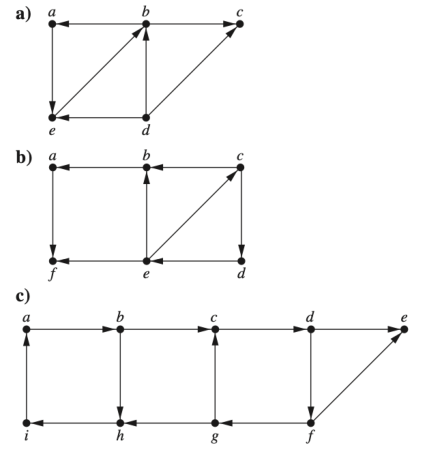
\includegraphics[width=0.4\linewidth]{q5_figure.pdf}
\end{figure}

\end{question}

\par\noindent\rule{\textwidth}{0.5pt}

\subsubsection*{Solutions}
\begin{enumerate}[label=\textbf{\alph*).}]
  \item (a, b, e), (d), (c)
  \item (a), (f), (b), (c, d, e)
  \item (a, b, c, d, f, g, h, i), (e)

\end{enumerate}
\newpage
\begin{question}
How many of the disjunctions $p \lor \neg q$, $\neg p \lor q$, $q \lor r$, $q \lor \neg r$, and $\neg q \lor \neg r$ can be made simultaneously true by an assignment of truth values to $p$, $q$, and $r$?
\end{question}

\par\noindent\rule{\textwidth}{0.5pt}

\subsubsection*{Solutions}

\begin{center}
\begin{tabular}[h]{|ccc|ccccc|r|}
    \hline
    p & q & r & $p \lor \neg q$ & $\neg p \lor q$ & $q \lor r$ & $q \lor \neg r$ & $\neg q \lor \neg r$ & correct \\
    \hline
    T & T & T & T & T & T & T & F & 4 \\
    T & T & F & T & T & T & T & T & 5 \\
    T & F & T & T & F & T & F & T & 3 \\
    T & F & F & T & F & F & T & T & 3 \\
    F & T & T & F & T & T & T & F & 3 \\
    F & T & F & F & T & T & T & T & 4 \\
    F & F & T & T & T & T & F & T & 4 \\
    F & F & F & T & T & F & T & T & 4 \\
    \hline
\end{tabular}
\end{center}

\noindent So, when $(p, q, r) = (T, T, F)$, all of the disjunctions can be true simultaneously. Therefore, the answer is \textbf{5}.
\newpage
\begin{question}
Determine the truth value of each of these statements if the domain consists of all real numbers.
\begin{enumerate}
    \item \(\exists x(x^3 = -1)\)
    \item \(\exists x(x^4 < x^2)\)
    \item \(\forall x((-x)^2 = x^2)\)
    \item \(\forall x(2x > x)\)
\end{enumerate}
\end{question}

\par\noindent\rule{\textwidth}{0.5pt}

\subsubsection*{Solutions}
\begin{enumerate}
    \item \textbf{True}. Let $x = -1$, then $x^3 = -1$. It exists at least one $x$ satisfiying the statement.
    \item \textbf{True}. Let's pick some $x$ bigger than 0 and smaller than 1. For example, $x = 0.1$. Then $x^4 = 0.0001$ and $x^2 = 0.01$. Therefore, it exists at least one $x$ satisfiying the statement.
    \item \textbf{True}. This is because square of any real number is always non-negative. Therefore, $(-x)^2 = x^2$ for all $x$.
    \item \textbf{False}. Let $x = -1$, then $2x = -2$ and $x = -1$. Then $-2 > -1$, which is false. Therefore, there are counterexamples for the statement.
\end{enumerate}


\newpage
\begin{question}
Express each of these system specifications using predicates, quantifiers, and logical connectives.
\begin{enumerate}
\item When there is less than 30 megabytes free on the hard disk, a warning message is sent to all users.
\item No directories in the file system can be opened and no files can be closed when system errors have been detected.
\item The file system cannot be backed up if there is a user currently logged on.
\item Video on demand can be delivered when there are at least 8 megabytes of memory available and the connection speed is at least 56 kilobits per second.
\end{enumerate}
\end{question}

\par\noindent\rule{\textwidth}{0.5pt}

\subsubsection*{Solutions}
\begin{enumerate}
    \item Let $P(x)$ be the predicates `There is less than 30 megabytes free on the hard disk $x$' and $Q(y)$ be the predicates `A warning message is sent to user $y$' Then, $$\exists x P(x) \rightarrow \forall y Q(y)$$
    \item Let $P(x)$ be the predicates `System error $x$ has been detected', $Q(y)$ be the predicates `Directory $y$ in the file system can be open', and $R(z)$ be the predicates `File $z$ can be closed'. Then, $$\exists x P(x) \rightarrow \forall y \forall z(\neg Q(y) \wedge \neg R(z))$$
    \item Let $P(x)$ be the predicates `User $x$ is currently logged on' and $Q(y)$ be the predicates `The file system $y$ can be backed up'. Then, $$ \exists x (P(x)) \rightarrow \forall y \neg Q(y)$$
    \item Let $P(x)$ be the predicates `There are at least 8 megabytes of memory $x$ available', $Q(y)$ be the predicates `The connection speed $y$ is at least 56 kilobits per second', and $R(x)$ be the predicates `Video on demand $z$ can be delivered'. Then, $$\exists x \exists y( P(x) \wedge Q(y)) \rightarrow \forall z R(z)$$
\end{enumerate}

\newpage
\begin{question}
Let F(x, y) be the statement “x can fool y,” where the domain consists of all people in the world. Use quantifiers to express each of these statements.
\begin{enumerate}
\item Everybody can fool Fred.
\item Evelyn can fool everybody.
\item Everybody can fool somebody.
\item There is no one who can fool everybody.
\item Everyone can be fooled by somebody.
\item No one can fool both Fred and Jerry.
\item Nancy can fool exactly two people.
\item There is exactly one person whom everybody can fool.
\item No one can fool himself or herself.
\item There is someone who can fool exactly one person besides himself or herself.
\end{enumerate}
\end{question}

\par\noindent\rule{\textwidth}{0.5pt}

\subsubsection*{Solutions}

\begin{enumerate}
    \item $\forall x F(x, \text{Fred})$
    \item $\forall x F(\text{Evelyn}, x$)
    \item $\forall x \exists y F(x, y)$
    \item $\neg \exists x \forall y F(x, y)$
    \item $\forall x \exists y F(y, x)$
    \item $\neg \exists x (F(x, \text{Fred})) \wedge (F(x, \text{Jerry}))$
    \item $\exists x \exists y (\neg(x = y) \wedge F(\text{Nancy}, x) \wedge F(\text{Nancy}, y) \wedge (\forall z (F(\text{Nancy}, z) \rightarrow (z = x \vee z = y))))$
    \item $\forall y (\exists x (F(x, y)) \wedge \exists z(F{z, y})) \rightarrow (x = z)$
    \item $ \neg \exists x F(x, x)$
    \item $\exists x \exists y (\neg(x = y) \wedge F(x, y) \wedge \neg \exists z (F(x, z) \wedge \neg(z = y)))$
\end{enumerate}

\newpage
\begin{question}
Let \( Q(x, y) \) be the statement "\( x + y = x - y \)". If the domain for both variables consists of all integers, what are the truth values?
\begin{enumerate}
\item \( Q(1, 1) \)
\item \( Q(2, 0) \)
\item \( \forall y Q(1, y) \)
\item \( \exists x Q(x, 2) \)
\item \( \exists x \exists y Q(x, y) \)
\item \( \forall x \exists y Q(x, y) \)
\item \( \exists y \forall x Q(x, y) \)
\item \( \forall y \exists x Q(x, y) \)
\item \( \forall x \forall y Q(x, y) \)
\end{enumerate}
\end{question}

\par\noindent\rule{\textwidth}{0.5pt}

\subsubsection*{Solutions}
\begin{enumerate}
    \item \textbf{False}. $ 1 + 1 = 1 - 1$ is not true.
    \item \textbf{True}. $ 2 + 0 = 2 - 0$ is true.
    \item \textbf{False}. There is counterexample such as $y = 1$. (Note Q10.1)
    \item \textbf{False}. There is no integer $x$ such that $x + 2 = x - 2$, $2 = -2$ is not true.
    \item \textbf{True}. For example, $x = 2, y = 0$. (Note Q10.2) So there is a pair $x, y$ $s.t.$ $Q(x, y)$ is true.
    \item \textbf{True}. There is $y (= 0)$ for which $Q(x, y)$ is true for every x.
    \item \textbf{True}. Let $y$ is $0$, then for every $x$, statement is true.
    \item \textbf{False}. There is $y$ $s.t.$ $Q(x, y)$ is not true for every $x$.
    \item \textbf{False}. There are countercases. (i.g. $x = 1, y = 1$)
\end{enumerate}

\end{document}